
\documentclass{beamer}

\mode<presentation> {

% The Beamer class comes with a number of default slide themes
% which change the colors and layouts of slides. Below this is a list
% of all the themes, uncomment each in turn to see what they look like.

%\usetheme{default}
%\usetheme{AnnArbor}
%\usetheme{Antibes}
%\usetheme{Bergen}
%\usetheme{Berkeley}
%\usetheme{Berlin}
%\usetheme{Boadilla}
%\usetheme{CambridgeUS}
%\usetheme{Copenhagen}
%\usetheme{Darmstadt}
%\usetheme{Dresden}
%\usetheme{Frankfurt}
%\usetheme{Goettingen}
%\usetheme{Hannover}
%\usetheme{Ilmenau}
%\usetheme{JuanLesPins}
%\usetheme{Luebeck}
\usetheme{Madrid}
%\usetheme{Malmoe}
%\usetheme{Marburg}
%\usetheme{Montpellier}
%\usetheme{PaloAlto}
%\usetheme{Pittsburgh}
%\usetheme{Rochester}
%\usetheme{Singapore}
%\usetheme{Szeged}
%\usetheme{Warsaw}

%\usecolortheme{albatross}
%\usecolortheme{beaver}
%\usecolortheme{beetle}
%\usecolortheme{crane}
%\usecolortheme{dolphin}
%\usecolortheme{dove}
%\usecolortheme{fly}
%\usecolortheme{lily}
%\usecolortheme{orchid}
%\usecolortheme{rose}
%\usecolortheme{seagull}
%\usecolortheme{seahorse}
%\usecolortheme{whale}
%\usecolortheme{wolverine}
}

\usepackage{graphicx}
\usepackage{booktabs}  
\usepackage[utf8]{vietnam}

\title[]{The world's hardest game\\ 
với phương pháp học tăng cường} 

\author{Phan Quang Khánh\\[0.5cm]{\small Người hướng dẫn:TS. Huỳnh Thế Đăng}} % Your name
\institute[] % Your institution as it will appear on the bottom of every slide, may be shorthand to save space
{
Trường đại học Khoa học Tự nhiên \\ % Your institution for the title page
\medskip
\textit{1611125@student.hcmus.edu.vn} % Your email address
}
\date{\today} % Date, can be changed to a custom date

\begin{document}

\begin{frame}
\titlepage % Print the title page as the first slide
\end{frame}

\begin{frame}
\frametitle{Overview}
\tableofcontents 
\end{frame}

\section{Đặt vấn đề}

\begin{frame}
\frametitle{Đặt vấn đề}
\begin{figure}[h]
    \centering
    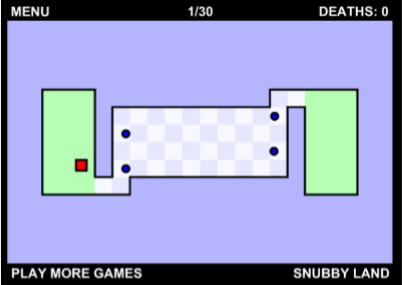
\includegraphics{photo/lv1game.png}
    \caption{Vòng đầu tiên của TWHG}
    \label{fig:my_label}
\end{figure}
\end{frame}

\begin{frame}
\frametitle{Đặt vấn đề}
\begin{figure}[h]
    \centering
    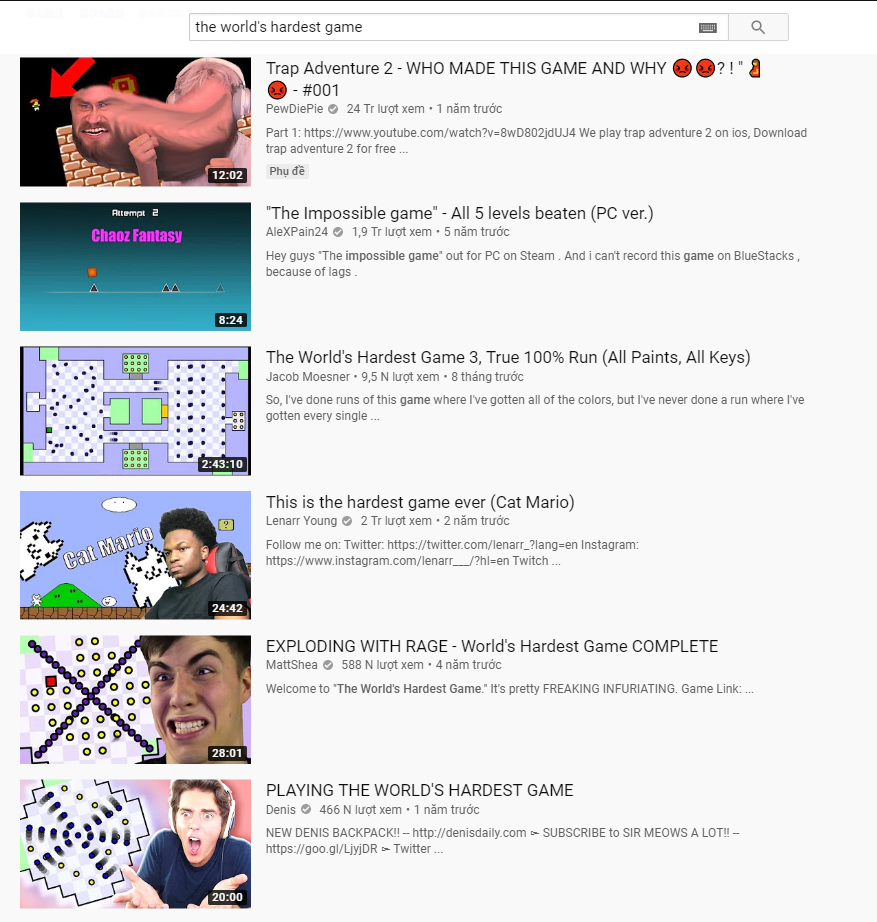
\includegraphics[scale=0.4]{photo/TWHG-react.png}
    \caption{Vòng đầu tiên của TWHG}
    \label{fig:my_label}
\end{figure}
\end{frame}

%------------------------------------------------
\section{Cơ sở lý thuyết}
\begin{frame}
\frametitle{Cơ sở lý thuyết}
\begin{itemize}
\item Học tăng cường
\item Học tăng cường chuyên sâu
\item Mô phỏng trò chơi
\end{itemize}
\end{frame}

\section{Hướng tiếp cận}
\begin{frame}
\frametitle{Hướng tiếp cận}
\begin{figure}[h]
    \centering
    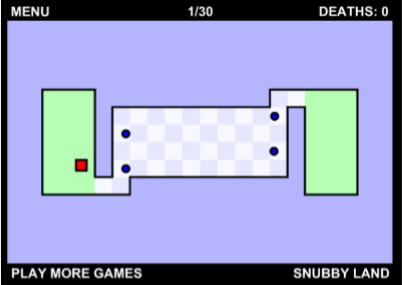
\includegraphics{photo/lv1game.png}
\end{figure}
\end{frame}

\subsection{Toy Games}
\begin{frame}
Như đã được trình bày ở trong phần trên, không thể huấn luyện mô hình trực tiếp từ mô phỏng của chính trò chơi. Do đó nhóm tác giả cho ra ba trò chơi nhỏ hơn nhằm mô phỏng lại trò chơi.
\frametitle{Toy games}
\begin{figure}[h]
    \centering
    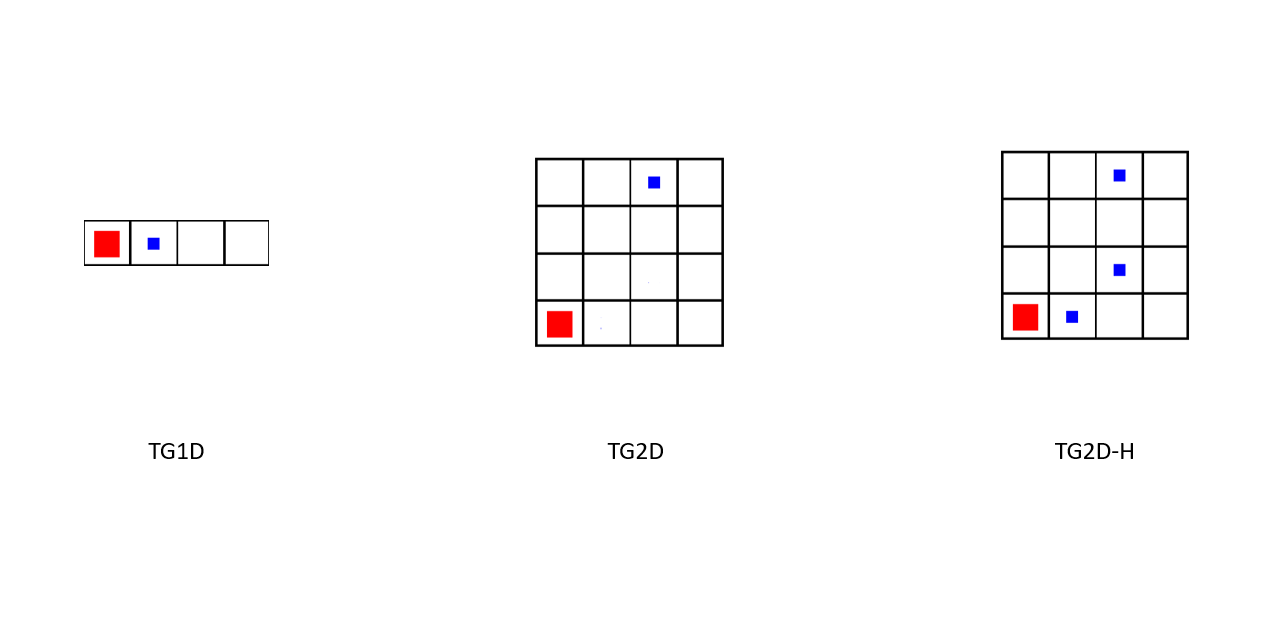
\includegraphics[scale=0.4]{photo/Toygame.png}
\end{figure}
\end{frame}

\begin{frame}
\frametitle{TG1D}
\begin{figure}[h]
    \centering
    
\includegraphics{photo/TG1D.png}
\end{figure}
\begin{block}{Vector trạng thái}
\begin{center}
\begin{align*}
S_x=\begin{cases}
-2\quad \quad &\text{khi $e=x$ và $p=x$}\\
-1\quad \quad &\text{khi $e=x$}\\
1 \quad \quad &\text{khi $p=x$}\\
0 \quad \quad &\text{trường hợp còn lại}
\end{cases}
\end{align*}
\end{center}
\end{block}
\end{frame}

\begin{frame}
\frametitle{TG2D}
\begin{figure}[h]
    \centering
    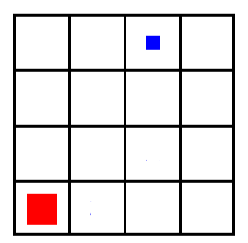
\includegraphics{photo/TG2D.png}
\end{figure}
\end{frame}

\begin{frame}
\frametitle{TG2D-H}
\begin{figure}[h]
    \centering
    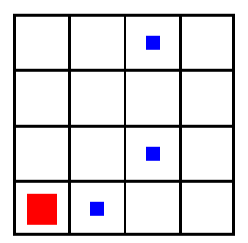
\includegraphics{photo/TG2D_H.png}
\end{figure}
\end{frame}


\subsection{Learning}
\begin{frame}
\frametitle{Learning}
Có thể thấy có 2 cách để xây dựng mô hình để giải quyết bài toán: sử dụng CNN để lấy thông tin rồi quyết định hành động cho trạng thái hoặc phân tách thành các vector trạng thái  và sử dụng mô hình FC.
\end{frame}
\begin{frame}
\frametitle{Learning}
\begin{block}{Mô hình huấn luyện}
Cấu trúc của mô hình được xây dựng như cấu trúc trong bài báo DeepMind, với đầu vào là hình ảnh của từng khung hình và số lượng 3 hoặc 5 node đầu ra, dựa trên trò chơi. Mô hình sử dụng mạng nơ-ron gồm 2 lớp ẩn được kết nối đầy đủ cho đầu vào là một vector trạng thái lần lượt có 128 và 64 ReLU node.\\
\end{block}
\begin{block}{Hàm mất mát}
\[\mathcal{L} = \dfrac{1}{|\mathcal{B}|}\sum_{t\in \mathcal{B}}\left[\left(Q(t,a_t) - \left[r_{t,a} + \gamma \max_{a\in \mathcal{A}} Q(t+1,a)\right]\right)\right]^2\]
\end{block}
\end{frame}

\begin{frame}
\frametitle{Learning}
\begin{figure}[t]
    \centering
    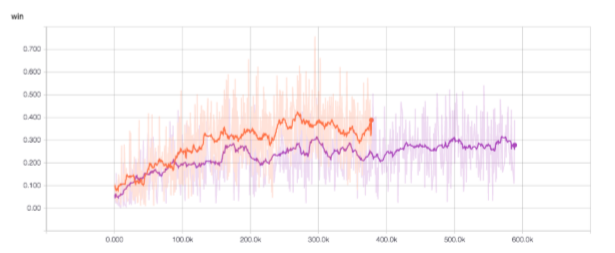
\includegraphics{photo/2model.png}
    \caption{Tỉ lệ thắng trong việc huấn luyện TG2D-H}
    \label{fig:my_label}
\end{figure}
\end{frame}

\subsection{Kết quả}
\begin{frame}
\frametitle{Kết quả}
Kết quả sau là được chạy 10 lượt, mỗi lượt chứa 1000 games, tất cả có 10,000 mẫu.\\
\textit{Random}: Thực hiện mô hình ngẫu nhiên là mô hình chính. Mô hình tạo mẫu của hành động theo phân phối chuẩn
\begin{figure}[h!]
    \centering
    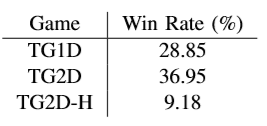
\includegraphics{photo/result1.png}
\end{figure}
\end{frame}

\begin{frame}
\frametitle{Kết quả}
\textit{$\epsilon$-Greedy}: Mô hình thứ 2 tạo mẫu hành động theo phân phối chuẩn với xác suất tạo là $\epsilon$ và chọn hành động tham lam tại $t+1$ dựa trên phần thưởng tại $t$ với xác suất $1-\epsilon$. Cụ thể sử dụng $\epsilon=0.05$
\\
\\
\begin{figure}[h]
    \centering
    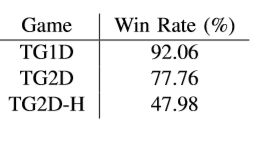
\includegraphics{photo/result2.png}
\end{figure}
\end{frame}

\section{Cơ hội và định hướng}
\begin{frame}
\frametitle{Cơ hội}
\textit{Mô phỏng trò chơi}\\
Nhóm tác giả sử dụng flash và trình duyệt để mô phỏng trò chơi làm cho thời gian huấn luyện mất nhiều thời gian hơn. Và sắp tới các trình duyệt cùng lúc bỏ flash nên việc thực hiện lại trên ý tưởng này là rất khó. Và nhóm tác giả không thể đưa ra được biễu diễn trực quan trên flash.\\
\end{frame}

\begin{frame}
\frametitle{Cơ hội}
\textit{Thời gian thực hiện}\\
Thời gian thực hiện của nhóm tác giả chưa đủ để có một bản báo cáo tốt như được trình bày ở trên. Do đó sự chuẩn bị trước cho luận văn tốt nghiệp giúp cho thời gian thực hiện đề tài hợp lý hơn.
\end{frame}

\begin{frame}
\frametitle{Cơ hội}
\textit{Mô phỏng trò chơi}
Nhóm tác giả sử dụng flash và trình duyệt để mô phỏng trò chơi làm cho thời gian huấn luyện mất nhiều thời gian hơn. Và sắp tới các trình duyệt cùng lúc bỏ flash nên việc thực hiện lại trên ý tưởng này là rất khó. Và nhóm tác giả không thể đưa ra được biễu diễn trực quan trên flash.\\
\end{frame}

\begin{frame}
\frametitle{Định hướng}
\textit{Mô phỏng trò chơi:} 
\begin{itemize}
    \item Nhóm đang can thiệp vào mã nguồn java của TWHG với mục đích tạo nhiều hơn một đối tượng để tìm kiếm phương án tốt hơn.
    \item Thay vì huấn luyện từng toy games theo cách ngãu nhiên, nhóm cố trích xuất không gian trò chơi và tạo thành các state vector để huấn luyện trực tiếp.
    \item Tùy biến các tham số cùng thay đổi vận tốc của chương trình để giúp việc huấn luyện nhanh hơn.
    \item Cố gắng tạo ra API có thể biểu diễn được chương trình.
\end{itemize} \\
\end{frame}

\begin{frame}
\frametitle{Định hướng}
\textit{Toy games:} \\
Có thể thấy kết quả của TG2D-H vẫn còn thấp nên việc tìm kiếm phương án biểu diễn tốt hơn. Ngoài ra, nhóm cho giả thiết rằng TG1D có thể đạt được kết quả tốt nhất nếu có thời gian huấn luyện nhiều hơn.\\
\end{frame}

\begin{frame}
\frametitle{Định hướng}
\textit{Thiết bị huấn luyện:}\\ Nhóm sẽ cố gắng tìm kiếm sự giúp đỡ của bộ môn hoặc thuê các máy chủ ảo để huấn luyện (Google Cloud, AWS, \dots).\\
\\
\end{frame}



\begin{frame}
\Huge{\centerline{The End}}
\end{frame}

%----------------------------------------------------------------------------------------

\end{document} 